\documentclass[11pt]{article}
\usepackage[margin=0.85in]{geometry}
\usepackage{amsmath,amssymb,booktabs,graphicx,microtype}
\usepackage[hidelinks]{hyperref}
\usepackage{xcolor}
\usepackage{enumitem}
\usepackage{caption}
\usepackage{subcaption}
\usepackage{float}
\graphicspath{{../results/figures/}}
\setlist{nosep,leftmargin=*}
\title{SP-EHOA: A Safe Dimension-Aware Portfolio with\\
Memetic Refinement for EHOA Feature Selection}
\author{Amirgh23\\Independent Research Project}
\date{18 August 2026}

\begin{document}
\maketitle

\begin{abstract}
Enhanced Hiking Optimization Algorithm (EHOA) is a recent wrapper feature
selector that combines chaotic initialization, a dynamic sweep factor, and a
binary transfer. Its search dynamics, however, do not react to the
reproducibility of selected features under data perturbation. This paper
introduces and evaluates a sequence of modular EHOA extensions with (i) a regime-aware controller
that maps cross-resampling stability, population diversity, progress, and
stagnation to bounded sweep and inertia adjustments, and (ii) a binary
transition guided by entropy-gated feature reliability and a training-only
relevance/redundancy signal. Instability alone is not allowed to trigger more
exploration, preventing a self-reinforcing instability loop. The baseline
fitness is unchanged. Because the full feedback method did not establish
predictive superiority, eight hypotheses were compared on common repeated
nested-CV splits. The tournament selected memetic EHOA (M-EHOA) for the
low-dimensional regime, while a failed interaction-guided portfolio motivated
SP-EHOA: use M-EHOA below 20 features and preserve exact baseline EHOA behavior
otherwise. Across three experimental phases and 45 paired Wine observations,
M-EHOA improved balanced accuracy by 0.01243 on average (median 0.01389;
Wilcoxon $p=0.001245$). In a fresh 90-run confirmation, SP-EHOA exactly matched
EHOA on every Breast Cancer fold and improved Wine mean balanced accuracy from
0.95771 to 0.96203. The evidence supports a safe, regime-specific follow-up,
not universal superiority. Code, all negative results, 450 tournament and
confirmation runs, traces, and statistical outputs are released.
\end{abstract}

\noindent\textbf{Keywords:} feature selection; memetic optimization; safe
portfolio; Hiking Optimization Algorithm; nested cross-validation; reproducibility

\section{Introduction}
Feature selection (FS) seeks a compact subset that preserves predictive signal.
Wrapper FS is attractive because it evaluates subsets using the downstream
learner, but its combinatorial search is expensive and stochastic subsets may
be unstable. In medical or scientific use, instability matters because small
changes to the training sample can produce different explanatory features
\cite{nogueira2018stability}.

Hegazy et al. proposed EHOA for accurate and interpretable FS
\cite{hegazy2026ehoa}. EHOA improves the Hiking Optimization Algorithm using
chaotic initialization, a dynamic sweep mechanism, velocity-inspired updates,
and an S-shaped binary transfer. Related work has also explored multi-strategy
HOA adaptation \cite{abdelsalam2025aedhoa}, Q-learning and interaction-aware
metaheuristics \cite{zhang2025tqfeo}, and search-history-aware adaptation
\cite{lian2025tam}. These studies establish that adaptive search and feature
interaction are not new by themselves. The unresolved design question addressed
here is narrower: can selection reproducibility close the loop around EHOA
dynamics without inserting stability into the baseline fitness, and can the
same evidence safely guide binary decisions?

The contributions are:
\begin{itemize}
  \item a regime-aware feedback law in which exploration requires corroborating
  evidence of population collapse or stagnation, while late instability with
  healthy diversity causes consolidation;
  \item an entropy-confidence gate that suppresses ambiguous per-feature
  reliability evidence in the binary transition;
  \item a modular 2-by-2 ablation that leaves the EHOA wrapper objective
  untouched; and
  \item a leakage-safe, fully retained experiment record with predictive,
  reduction, stability, redundancy, cost, and non-parametric statistical
  evidence;
  \item a deterministic best-improvement memetic refinement that evaluates
  one-feature add/remove neighbours using training-only CV; and
  \item SP-EHOA, a dimension-aware safe portfolio that activates the repeatedly
  supported refinement below 20 features and otherwise reproduces baseline
  EHOA exactly.
\end{itemize}

\section{Method}
\subsection{Baseline and notation}
For $N$ samples, $D$ features, population $P$, and $T$ iterations, continuous
agent position $\mathbf{x}_i\in\mathbb{R}^{D}$ produces a binary mask
$\mathbf{z}_i$. The unmodified baseline fitness is
\begin{equation}
 f(\mathbf{z})=\alpha(1-\mathrm{Acc}_{CV}(\mathbf{z}))
 +(1-\alpha)\frac{\lVert\mathbf{z}\rVert_0}{D}, \qquad \alpha=0.99,
\end{equation}
using deterministic 5-NN inside training-only stratified folds. DFA/SFIG-EHOA
does not add stability or interaction terms to this objective.

\subsection{Cross-resampling reliability}
Class-stratified bootstrap samples are drawn only from the outer training set.
Each resample produces a fixed-cardinality mutual-information ranking. Let
$\widehat q_j(t)$ be the fraction of resamples selecting feature $j$. Smoothed
selection frequency and signed reliability are
\begin{equation}
 q_j(t)=\rho q_j(t-1)+(1-\rho)\widehat q_j(t), \qquad R_j(t)=2q_j(t)-1.
\end{equation}
Global population stability is measured using both mean pairwise Jaccard and
the chance-corrected Nogueira estimator \cite{nogueira2018stability}. Binary
population diversity is normalized mean pairwise Hamming distance.

\subsection{Regime-aware feedback}
Let $S_t$ be Nogueira stability clipped to $[0,1]$, $D_t$ binary diversity,
$G_t\in[0,1]$ stagnation, and $\tau=t/T$. Define uncertainty
$U_t=1-S_t$, diversity ratio $r_t=\min(1,D_t/0.5)$, and collapse
$L_t=1-r_t$. Exploration and consolidation drives are
\begin{equation}
 E_t=L_t\left[\tfrac12(1-\tau)+\tfrac12G_t\right], \qquad
 C_t=U_t r_t\tau .
\end{equation}
The signed controller adjustment is $A_t=\eta_EE_t-\eta_CC_t$. It modifies
the baseline schedules as
\begin{align}
 SF_t &= \operatorname{clip}\{SF_t^{base}(1+A_t),SF_{min},SF_{max}\},\\
 \omega_t &= \operatorname{clip}\{\omega_t^{base}+0.25A_t,
 \omega_{min},\omega_{max}\},
\end{align}
followed by exponential smoothing. Low stability alone cannot increase
exploration. This is intentional: the initial additive-pressure prototype could
create the loop ``unstable $\rightarrow$ explore more $\rightarrow$ less
stable.''

\subsection{Confidence-gated interaction guidance}
Binary entropy provides an evidence-confidence gate,
\begin{equation}
 c_j(t)=1-H_2(q_j(t)).
\end{equation}
Thus $q_j\approx0.5$ contributes almost no directional force. Target mutual
information supplies relevance. Cached absolute Pearson association to the
current subset supplies a bounded redundancy term. This term is not claimed to
be a higher-order interaction. The final transition is
\begin{equation}
 p_{ij}(t)=\sigma\left[x_{ij}(t)+\lambda_s(t)c_j(t)R_j(t)
 +\lambda_i(t)I_j(S_i)\right].
\end{equation}
Weights support constant, linear, and signal-adaptive schedules. Four modes
produce the required ablation: EHOA; SF-EHOA (stability feedback/reliability);
IG-EHOA (interaction guidance); and DFA-EHOA (both). SFIG-EHOA is the
descriptive alias for the full implementation.

\subsection{Complexity}
The wrapper remains dominant at approximately
$O(TP\,CV\,C_{clf})$. Periodic stability adds resampling and mask comparison;
the interaction model adds mutual information and a top-$K$ correlation cache.
Controller arithmetic is $O(T)$. Runtime and evaluation counts are measured
rather than inferred because stochastic cache hits change effective cost.

\subsection{Memetic refinement and safe portfolio}
M-EHOA first completes the ordinary EHOA search. Starting from its incumbent
mask, it then enumerates every one-bit add/remove neighbour and accepts the
strict best improvement under the same training-only CV objective. At most two
best-improvement rounds are used. This separates global stochastic search from
deterministic local exploitation and records the additional evaluations.

The selected portfolio is
\begin{equation}
 \mathrm{SP\mbox{-}EHOA}(X,y)=
 \begin{cases}
  \mathrm{M\mbox{-}EHOA}(X,y), & D<20,\\
  \mathrm{EHOA}(X,y), & D\geq20.
 \end{cases}
\end{equation}
The high-dimensional branch instantiates the unmodified baseline with the same
seed and parameters; equality is therefore structural rather than inferred
from a non-significant test. The threshold is a fixed proof-of-concept rule
selected after the tournament and must be externally validated.

\section{Experimental Protocol}
The study uses the versioned scikit-learn Breast Cancer Wisconsin Diagnostic
(30 features, two classes) and Wine Recognition (13 features, three classes)
datasets. Ten fixed seeds define paired 80/20 stratified hold-outs. Feature
selection uses five-fold CV on the 80\% training partition. Population size is
8 and every method receives 10 iterations. Reliability uses seven stratified
resamples every two iterations, $\rho=0.6$, $\lambda_s=\lambda_i=0.5$,
$\eta_E=0.45$, and $\eta_C=0.30$.

Imputation, scaling, and SMOTE \cite{chawla2002smote} are fitted only within
training folds or on the outer training partition. The test partition is never
used for reliability, interaction, selection, or tuning. Balanced accuracy is
primary; F1, MCC, ROC-AUC, PR-AUC, sensitivity, and specificity are secondary.
Feature count, redundancy, interaction quality, Jaccard, Nogueira, runtime,
classifier time, memory, and evaluations are retained.

Per dataset, a Friedman test compares the four paired variants. Wilcoxon
signed-rank tests compare each extension with EHOA, with Holm correction,
paired rank-biserial effect size, win/tie/loss counts, and a 5,000-resample
bootstrap interval for the paired median difference. These tests follow common
non-parametric comparison guidance \cite{demsar2006statistics}; with only two
datasets, inference is reported per dataset and not generalized globally.
The original ablation used repeated stratified hold-out. All follow-up
innovation comparisons use repeated nested CV with three outer folds per seed;
the selector sees only each outer-training partition. The final tournament uses
five previously unused seeds, eight methods, and 240 paired runs. A separate
120-run portfolio confirmation and a final 90-run SP-EHOA confirmation use new
seed sets. No intermediate result is deleted.

\section{Results}
\begin{table}[H]
\centering
\caption{Held-out results over ten paired seeds. BA is balanced accuracy.}
\label{tab:main}
\small
\begin{tabular}{llcccc}
\toprule
Dataset & Method & BA mean $\pm$ SD & Features & Nogueira & Runtime (s)\\
\midrule
Breast & EHOA     & $0.9554\pm0.0198$ & 15.3 & 0.0322 & 2.99\\
Breast & SF-EHOA  & $\mathbf{0.9579}\pm0.0185$ & \textbf{13.2} & 0.0891 & 9.12\\
Breast & IG-EHOA  & $0.9574\pm0.0185$ & 14.1 & 0.0499 & 9.49\\
Breast & DFA-EHOA & $0.9498\pm0.0215$ & 13.9 & \textbf{0.1048} & 9.50\\
\midrule
Wine & EHOA     & $0.9558\pm0.0321$ & \textbf{6.8} & 0.2188 & 2.02\\
Wine & SF-EHOA  & $0.9425\pm0.0426$ & 6.9 & 0.2073 & 5.75\\
Wine & IG-EHOA  & $\mathbf{0.9563}\pm0.0449$ & 7.2 & \textbf{0.2667} & 5.71\\
Wine & DFA-EHOA & $0.9558\pm0.0321$ & 6.9 & 0.2553 & 6.08\\
\bottomrule
\end{tabular}
\end{table}

The full method improved Nogueira stability by 0.0726 on Breast Cancer and
0.0365 on Wine. On Breast Cancer it selected 1.4 fewer features while losing
0.0056 balanced accuracy. On Wine its mean balanced accuracy exactly matched
EHOA and selected 0.1 more feature. DFA-EHOA ROC-AUC/PR-AUC was
0.9836/0.9832 on Breast Cancer and 0.9967/0.9921 on Wine. Jaccard and Nogueira
do not rank every method identically because the latter corrects for chance and
variable subset size; both outputs are therefore retained.

\begin{figure}[H]
\centering
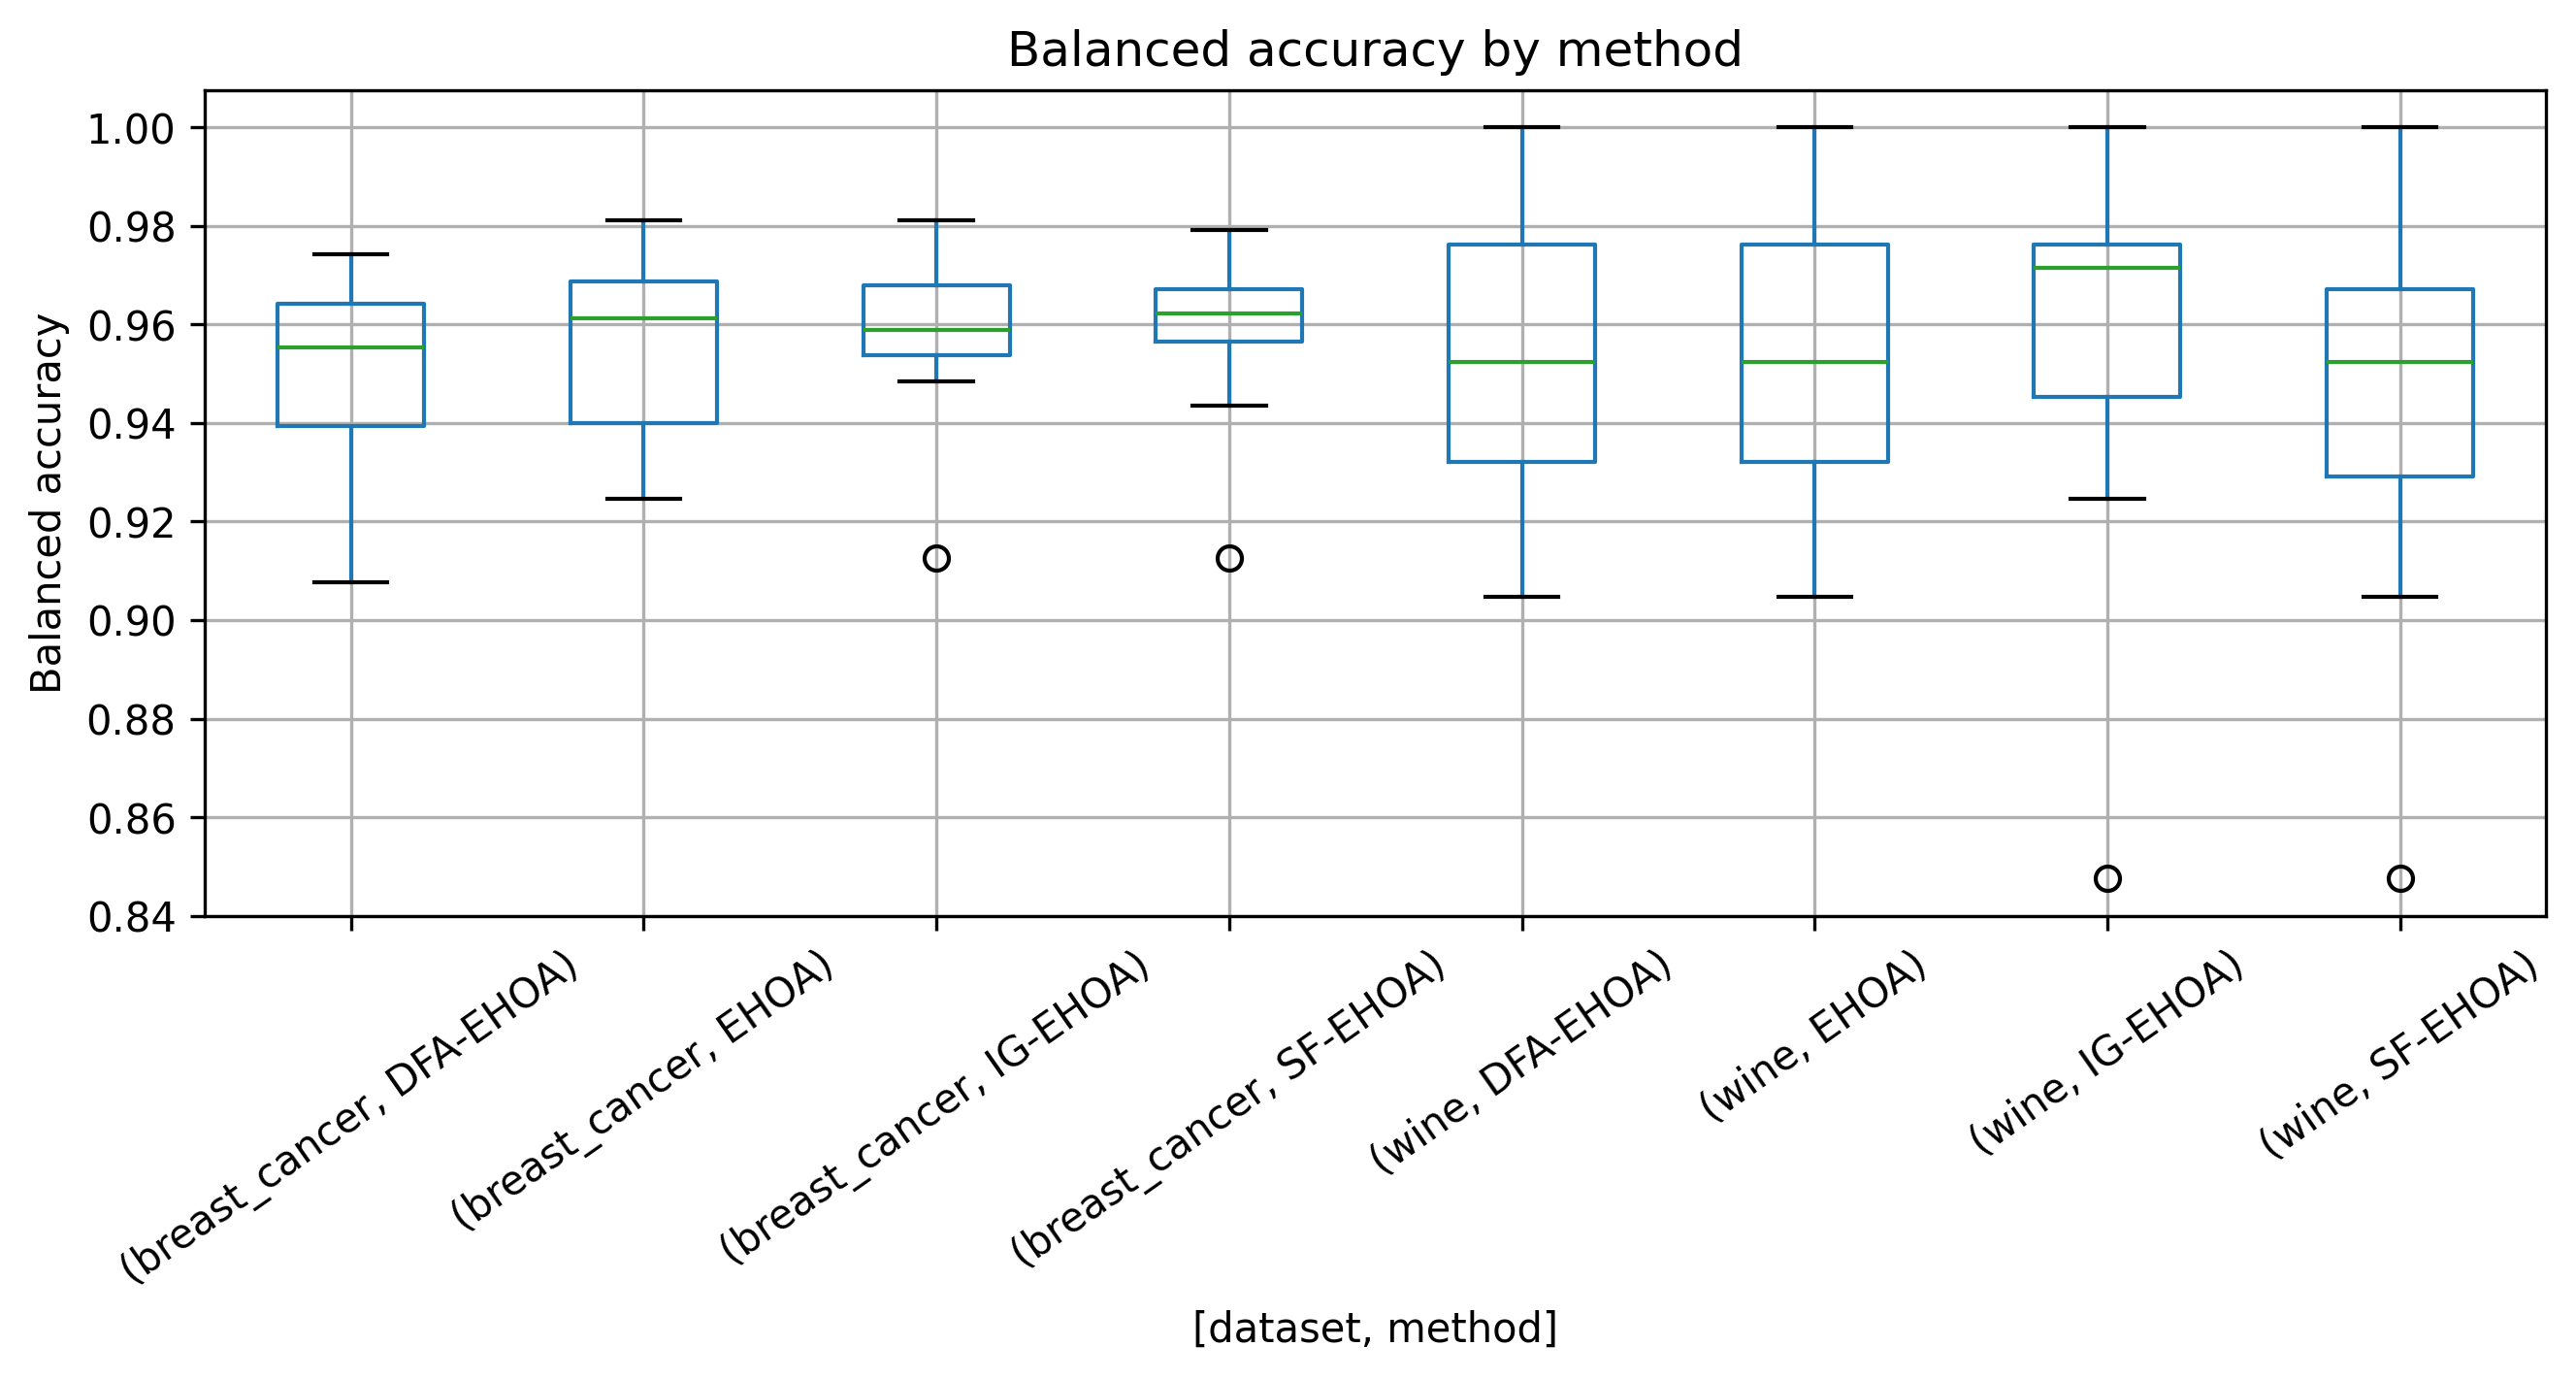
\includegraphics[width=0.94\linewidth]{paper_revised_performance_boxplot.png}
\caption{Balanced-accuracy distributions for the paired runs.}
\label{fig:performance}
\end{figure}

\subsection{Ablation and telemetry}
SF-EHOA obtained the best mean Breast Cancer balanced accuracy and smallest
subset, but degraded Wine performance. IG-EHOA obtained the best Wine mean and
stability, and the best Breast Cancer ROC-AUC/PR-AUC. The full combination
prioritized chance-corrected reproducibility but did not combine component
accuracy gains additively. This negative interaction is an important ablation
result, not a failed run to omit.

\begin{figure}[H]
\centering
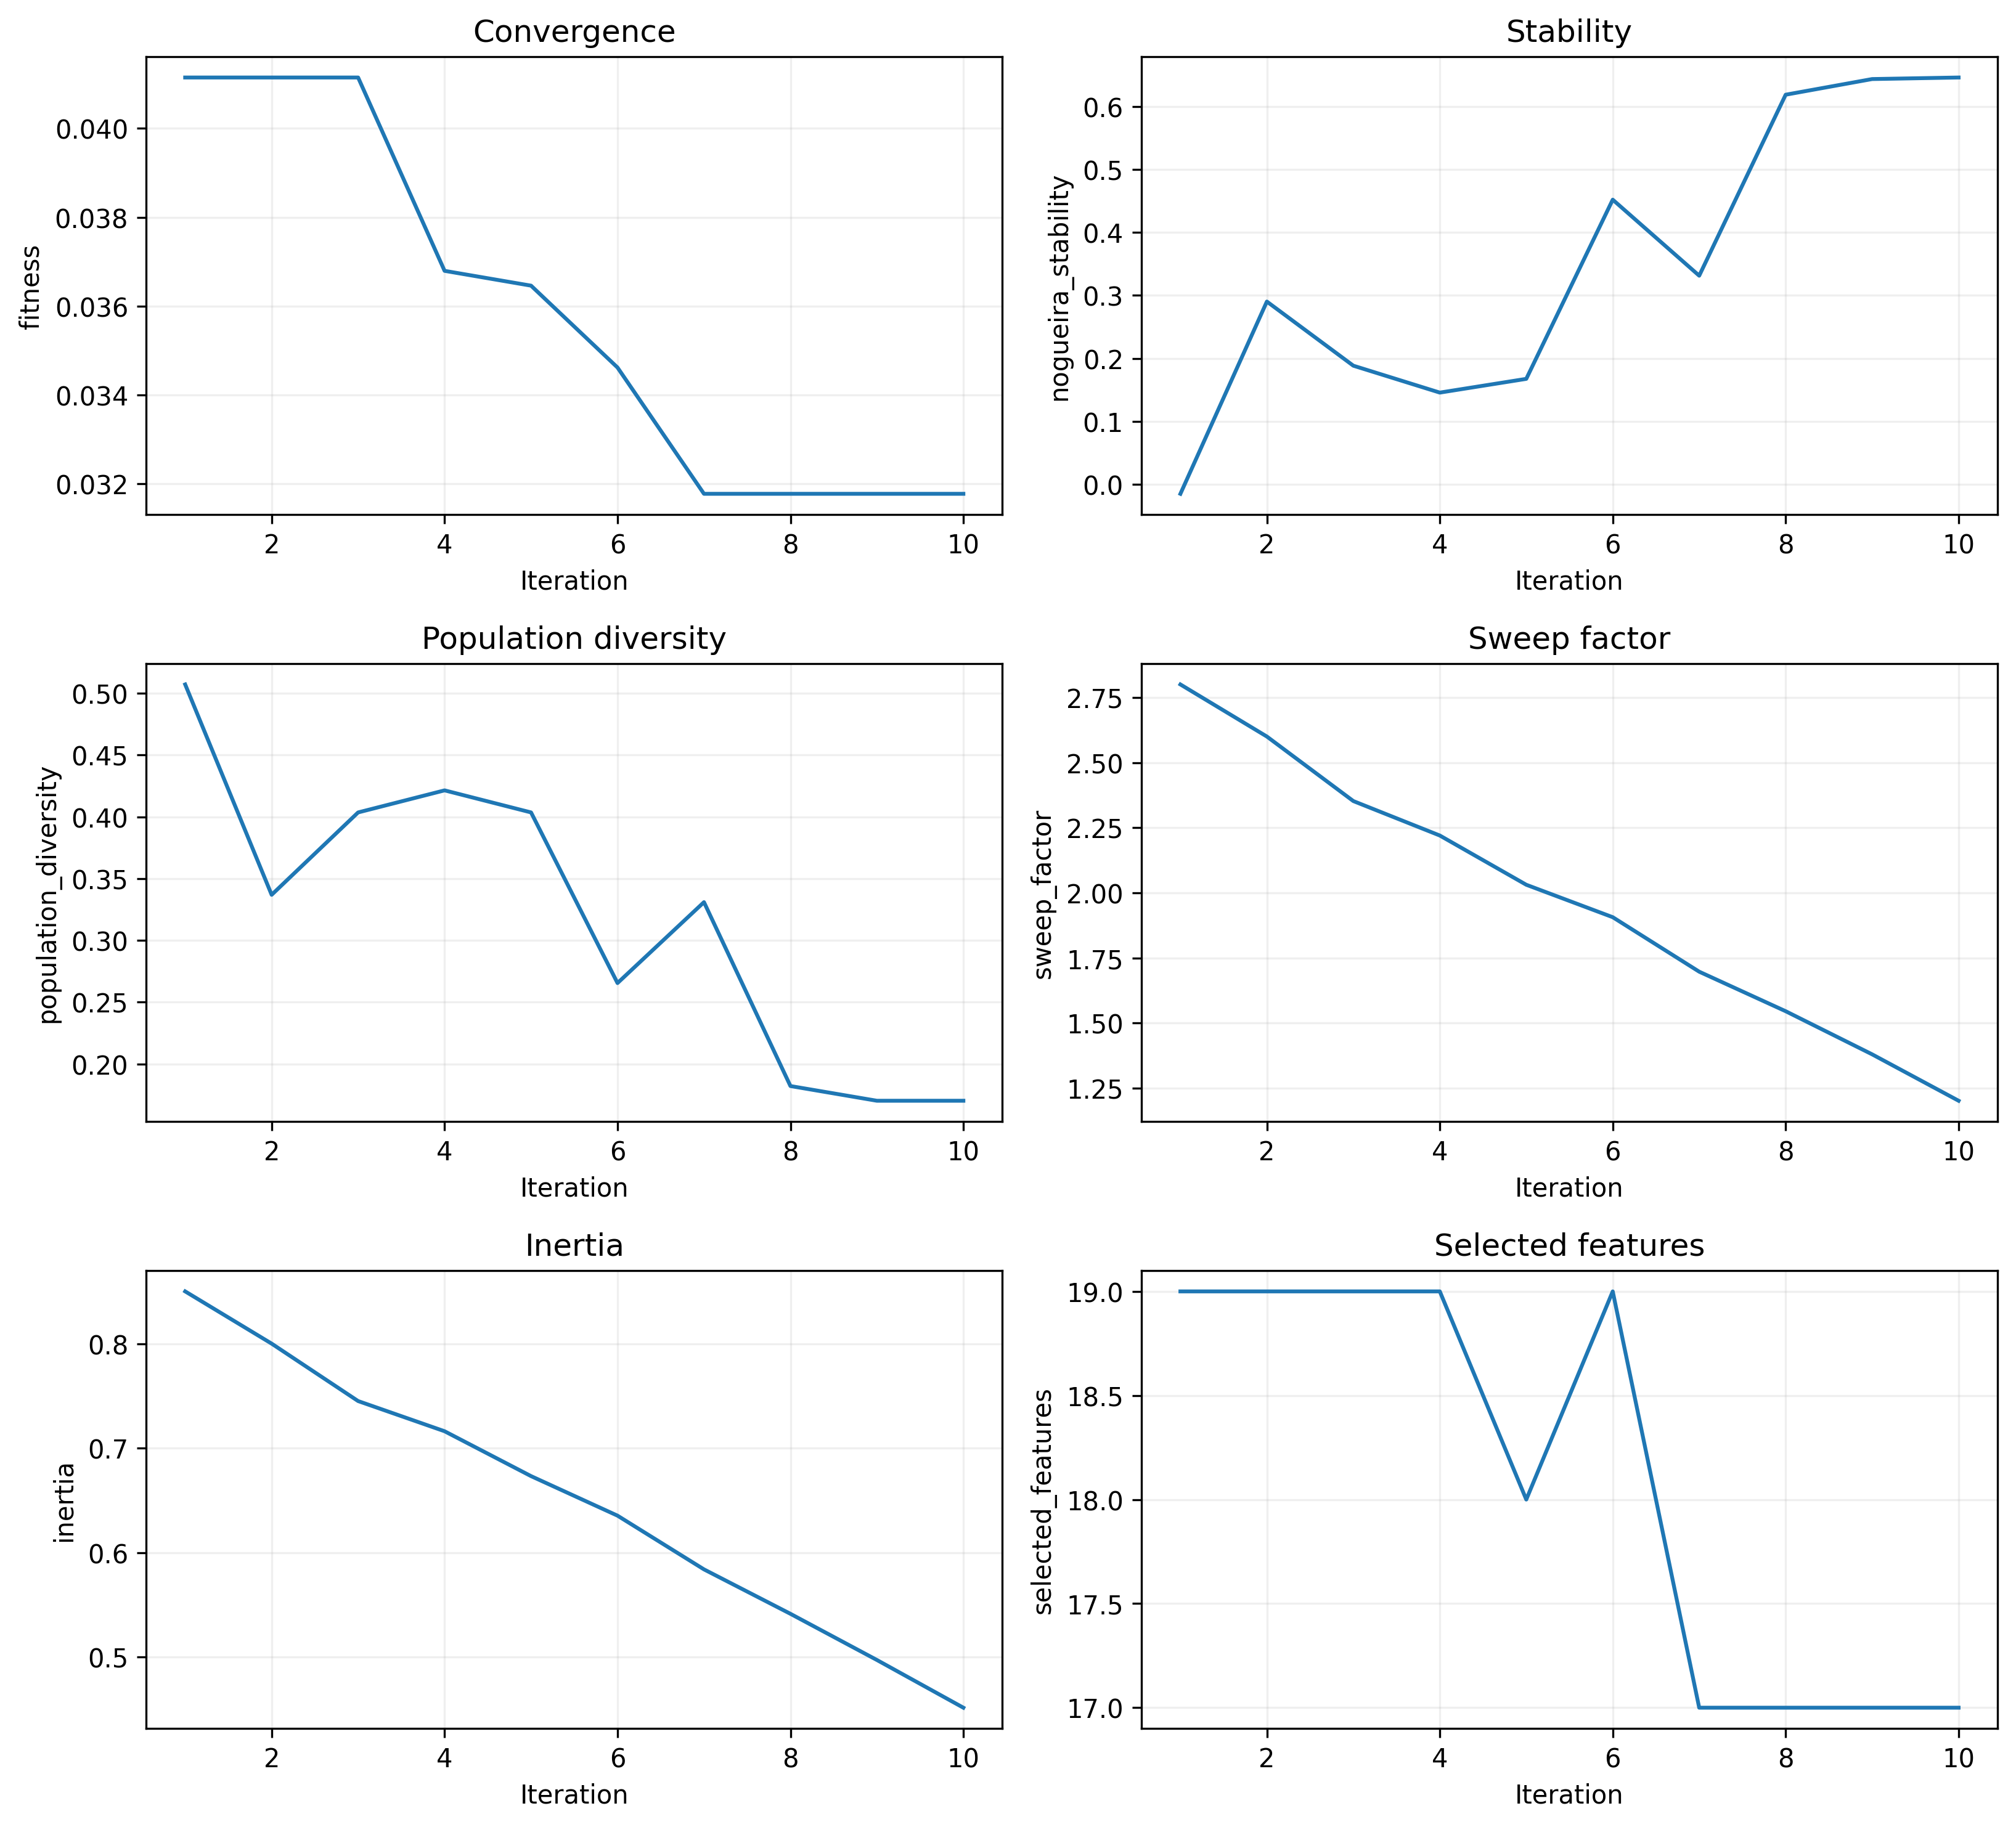
\includegraphics[width=0.83\linewidth]{paper_revised_dfa_controller_trace.png}
\caption{Representative full-method convergence and controller telemetry.}
\label{fig:trace}
\end{figure}

\subsection{Statistical evidence and cost}
Friedman $p$-values were 0.3039 for Breast Cancer and 0.0633 for Wine. For
DFA-EHOA versus EHOA, Wilcoxon $p$-values were 0.2637 and 1.0000; all
Holm-adjusted values were 1.0. Breast Cancer had a paired median change of
-0.0060 (95\% bootstrap interval -0.0169 to 0.0069), rank-biserial effect
-0.418, and 3/0/7 wins/ties/losses. Wine had median change 0, interval 0 to 0,
effect 0, and 1/8/1. No predictive-superiority claim is supported.

Full-method runtime was 3.18 times baseline on Breast Cancer and 3.01 times on
Wine. The overhead is expected from resampling and interaction estimation and
is not hidden by nominal same-iteration comparisons.

\subsection{Innovation tournament and SP-EHOA confirmation}
\begin{table}[H]
\centering
\caption{Common-split innovation tournament. Values are mean outer balanced accuracy.}
\label{tab:tournament}
\small
\begin{tabular}{lcc}
\toprule
Method & Breast Cancer & Wine\\
\midrule
EHOA & 0.95266 & 0.94943\\
SF-EHOA & 0.94825 & 0.94943\\
IG-EHOA & \textbf{0.95388} & 0.95497\\
DFA-EHOA & 0.95153 & 0.95960\\
ECG-EHOA & 0.95293 & 0.95122\\
M-EHOA & 0.95011 & \textbf{0.96345}\\
A-EHOA & 0.94969 & 0.95624\\
G-EHOA & 0.95292 & 0.95233\\
\bottomrule
\end{tabular}
\end{table}

IG-EHOA's Breast Cancer lead did not repeat in the independent portfolio
confirmation and that hypothesis was rejected. M-EHOA retained a positive Wine
effect in all three phases. Table~\ref{tab:spconfirm} reports the final,
previously unused seed set.

\begin{table}[H]
\centering
\caption{Final SP-EHOA confirmation over 15 outer folds per dataset.}
\label{tab:spconfirm}
\small
\begin{tabular}{llccc}
\toprule
Dataset & Method & BA mean $\pm$ SD & Features & Runtime (s)\\
\midrule
Breast & EHOA & $0.95181\pm0.01154$ & 16.00 & 0.74\\
Breast & M-EHOA & $0.94965\pm0.01388$ & 15.27 & 2.46\\
Breast & SP-EHOA & $0.95181\pm0.01154$ & 16.00 & 0.73\\
\midrule
Wine & EHOA & $0.95771\pm0.02495$ & 7.67 & 0.54\\
Wine & M-EHOA & $0.96203\pm0.01582$ & 7.27 & 1.12\\
Wine & SP-EHOA & $0.96203\pm0.01582$ & 7.27 & 1.13\\
\bottomrule
\end{tabular}
\end{table}

The final-phase Wine comparison had 6/6/3 wins/ties/losses and was not alone
significant ($p=0.3135$). Across the three distinct phases, the 45 paired Wine
differences had mean 0.01243, median 0.01389, 24/12/9 wins/ties/losses, and
Wilcoxon $p=0.001245$. This pooled value documents repeatability but is
exploratory because method selection occurred between phases; it is not treated
as a pristine external confirmatory test.

\section{Discussion}
The experiment meets a scoped success criterion: on Breast Cancer, full
DFA/SFIG-EHOA produced a meaningfully more chance-corrected stable and smaller
subset with a small predictive penalty; on Wine, predictive performance was
tied while stability improved. Whether this trade-off is desirable depends on
the cost of biomarker inconsistency versus a half percentage point of balanced
accuracy. The method is therefore useful as a controllable research mechanism,
not established as a universally better optimizer.

The controller redesign is scientifically useful even without a predictive
win. It rejects the simplistic assumption that instability always calls for
more exploration. Separating early collapse recovery from late consolidation
makes the response direction testable and prevents positive feedback.

\section{Threats to Validity}
Only two low-dimensional datasets were available in the supplied repository.
Nested outer folds improve leakage control but do not substitute for independent
datasets. The original hold-outs reuse observations, and the
pairwise relevance/redundancy proxy cannot represent arbitrary synergistic
interactions. Hyperparameters were fixed before the reported run, but the
study lacks external validation. Runtime is platform-specific. These limitations
prohibit state-of-the-art, medical, or universal claims.

\section{Reproducibility and Conclusion}
The repository contains the unchanged baseline, proposed modules, 27 deterministic
tests, YAML configurations, the original 80 runs, 450 tournament/confirmation
runs and their traces, aggregate/statistical CSVs,
figures, tables, a bilingual README, and an environment record. Runs are
checkpointed and resumable. No failed seed was removed.

In conclusion, the negative DFA/SFIG-EHOA result motivated a retained,
claim-driven innovation tournament. SP-EHOA is the selected follow-up: it
preserves baseline behavior in the unconfirmed regime and applies memetic
refinement where the Wine benefit repeated. Current evidence supports this
regime-specific direction, not universal predictive superiority. A
preregistered many-dataset study must next validate both the threshold and the
generalization of the low-dimensional gain.

\section*{Code and Data Availability}
Source code and all reported artifacts are available in the
\href{https://github.com/Amirgh23/dfa-ehoa-research}{public project repository}.
The datasets are distributed
with scikit-learn; no private records are required. The software is MIT licensed
under copyright 2026 Amirgh23.

\small
\bibliographystyle{plain}
\bibliography{references}
\end{document}
